In this section, we will review the results obtained with the model under default conditions. Those conditions are synthesized hereafter :

\begin{multicols}{3}
    \begin{itemize}
        \setlength\itemsep{0em}
        \item $P_e = 288 MW$
        \item $\eta_{pump} = 0.85$
        \item $\eta_{mec} = 0.98$
        \item $\eta_{is\_LP} = 0.90$
        \item $\eta_{is\_IP} = 0.90$
        \item $\eta_{is\_HP} = 0.92$
        \item $T_{drum} = 421.85K$
        \item $T_{max} = 838.15K$
        \item $T_{cd\_out} = 305.15K$
        \item $T_{cd\_subcool} = 1K$
        \item $p_3 = 31 MPa$
        \item $p_4 = 7 MPa$
    \end{itemize}
    \end{multicols}

\subsection{Table of the states obtained}


\begin{center}
\begin{longtable}{|c|c|c|c|c|c|c|}
    \hline
    States & $t \text{ } [^\circ C]$ & $p \text{ } [kPa]$ & $x \text{ } [-]$ & $h \text{ } [kJ/kg]$ & $s \text{ } [kJ/kgK]$ & $e \text{ } [kJ/kg]$\\
    \hline
    \endhead
    \hline
    \endfoot
    $1$ & $285.8$ & $10000$ & - & $1265.6$ & $3.112$ & $370.6$ \\
    $2$ & $293.5$ & $35000$ & - & $1295.1$ & $3.105$ & $401.9$ \\
    $3$ & $565.0$ & $31000$ & - & $3320.7$ & $6.077$ & $1571.1$ \\
    $4$ & $330.8$ & $7000$ & - & $2955.5$ & $6.130$ & $1190.6$ \\
    $5$ & $565.0$ & $6200$ & - & $3574.7$ & $7.056$ & $1543.0$ \\
    $6_{VII}$ & $485.0$ & $3751$ & - & $3414.7$ & $7.080$ & $1376.2$ \\
    $6_{VI}$ & $404.0$ & $2148$ & - & $3254.7$ & $7.106$ & $1208.6$ \\
    $6_{V}$ & $321.8$ & $1147$ & - & $3094.7$ & $7.136$ & $1039.9$ \\
    $6_{IV}$ & $238.4$ & $558$ & - & $2934.6$ & $7.172$ & $869.7$ \\
    $6_{III}$ & $154.1$ & $239$ & - & $2774.6$ & $7.214$ & $697.6$ \\
    $6_{II}$ & $95.6$ & $86$ & $0.98$ & $2614.6$ & $7.262$ & $523.7$ \\
    $6_I$ & $66.8$ & $27$ & $0.93$ & $2454.6$ & $7.314$ & $348.6$ \\
    $6$ & $33.0$ & $5$ & $0.89$ & $2294.5$ & $7.521$ & $128.9$ \\
    $7$ & $32.0$ & $5$ & $0.00$ & $134.1$ & $0.464$ & $1.9$ \\
    $9_{VII}$ & $246.6$ & $10000$ & - & $1069.4$ & $2.748$ & $279.2$ \\
    $9_{VI}$ & $216.0$ & $10000$ & - & $927.8$ & $2.467$ & $218.5$ \\
    $9_V$ & $185.9$ & $10000$ & - & $793.6$ & $2.184$ & $165.9$ \\
    $9_{IV}$ & $149.9$ & $10000$ & - & $637.8$ & $1.831$ & $111.9$ \\
    $7_{IV}$ & $148.7$ & $460$ & $0.00$ & $626.6$ & $1.829$ & $101.3$ \\
    $9_{III}$ & $125.9$ & $460$ & - & $529.1$ & $1.591$ & $72.2$ \\
    $9_{II}$ & $95.6$ & $460$ & - & $400.7$ & $1.257$ & $40.3$ \\
    $9_I$ & $66.8$ & $460$ & - & $279.9$ & $0.915$ & $17.8$ \\
    $8$ & $32.0$ & $460$ & - & $134.6$ & $0.464$ & $2.4$ \\
\end{longtable}
\end{center}

\vspace*{-1cm}

\subsection{T-s and h-s diagrams}
The T-s and h-s diagrams in default operating conditions are shown in figures \ref{fig:Ts_diagram} and \ref{fig:hs_diagram} respectively.
    
\begin{figure}[H]
    \centering
    % First figure
    \begin{minipage}{0.48\textwidth}
        \centering
        
\includegraphics[width=0.9\textwidth]{Figures/Ts_diagram.png}
        \caption{T-s diagram}
        \label{fig:Ts_diagram}
    \end{minipage}
    \hfill
    % Second figure
    \begin{minipage}{0.48\textwidth}
        \centering
        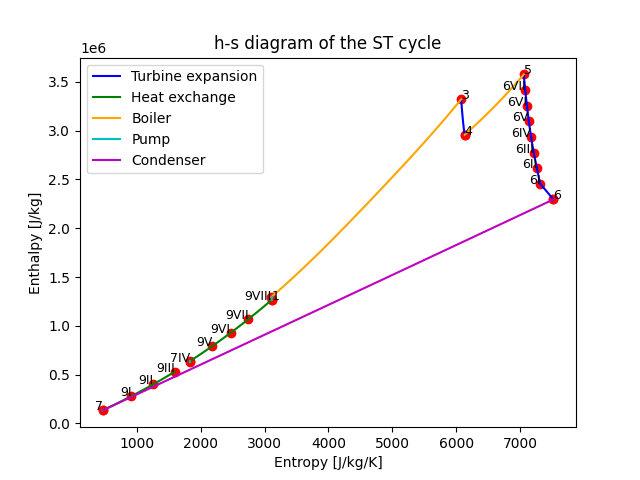
\includegraphics[width=0.9\textwidth]{Figures/hs_diagram.png}
        \caption{h-s diagram}
        \label{fig:hs_diagram}
    \end{minipage}
\end{figure}


\subsection{Energy and exergy pie charts}

The energy and exergy pie charts in default operating conditions are shown in figures \ref{fig:energy_pie_chart} and \ref{fig:exergy_pie_chart} respectively.

\begin{figure}[H]
    \centering
    % First figure
    \begin{minipage}{0.45\textwidth}
        \centering
        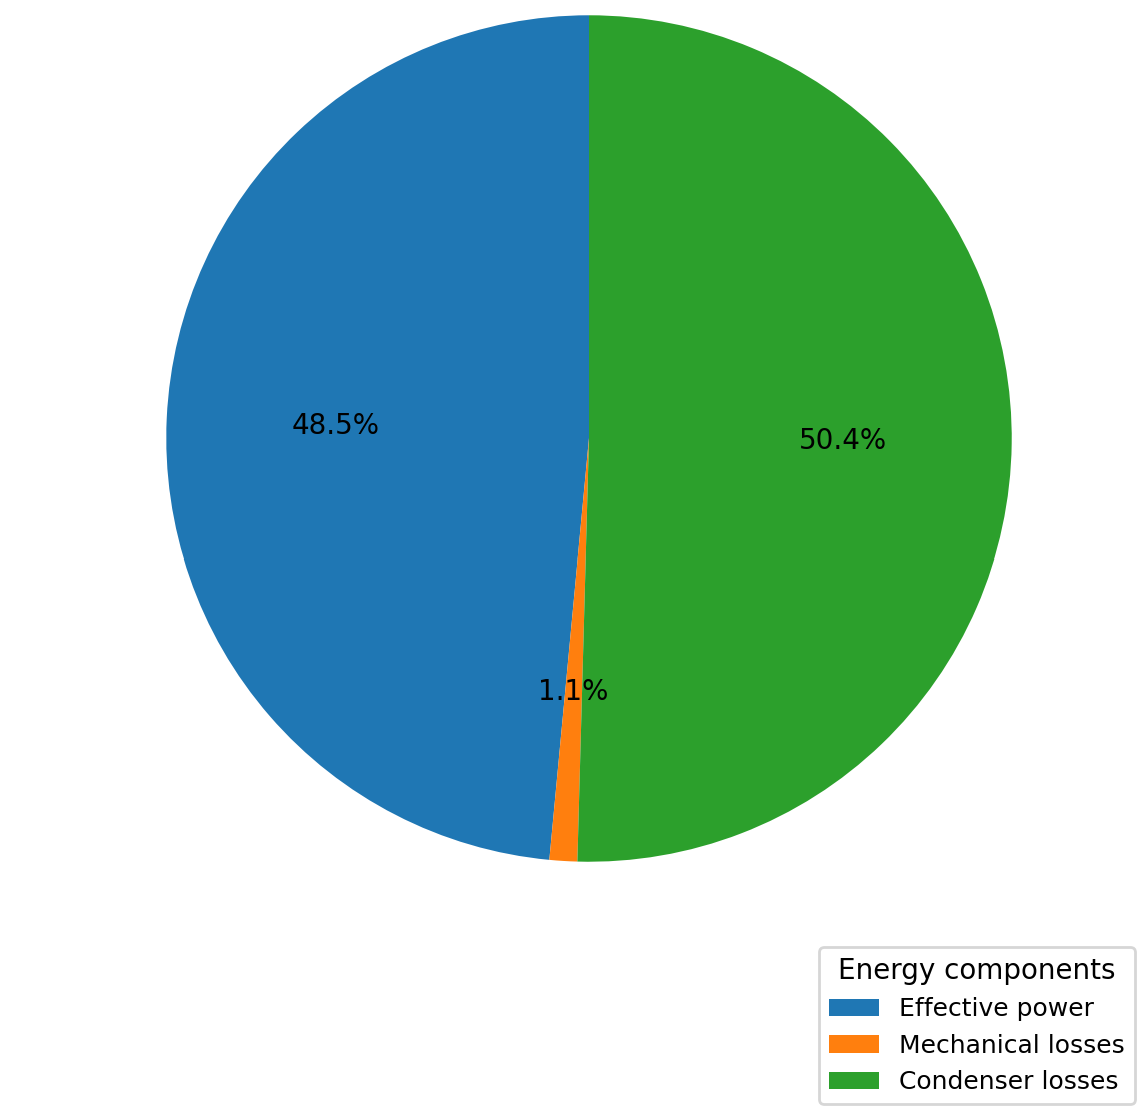
\includegraphics[width=0.7\textwidth]{Figures/pie_energy.png}
        \caption{Energy pie chart}
        \label{fig:energy_pie_chart}
    \end{minipage}
    \hfill
    % Second figure
    \begin{minipage}{0.43\textwidth}
        \centering
        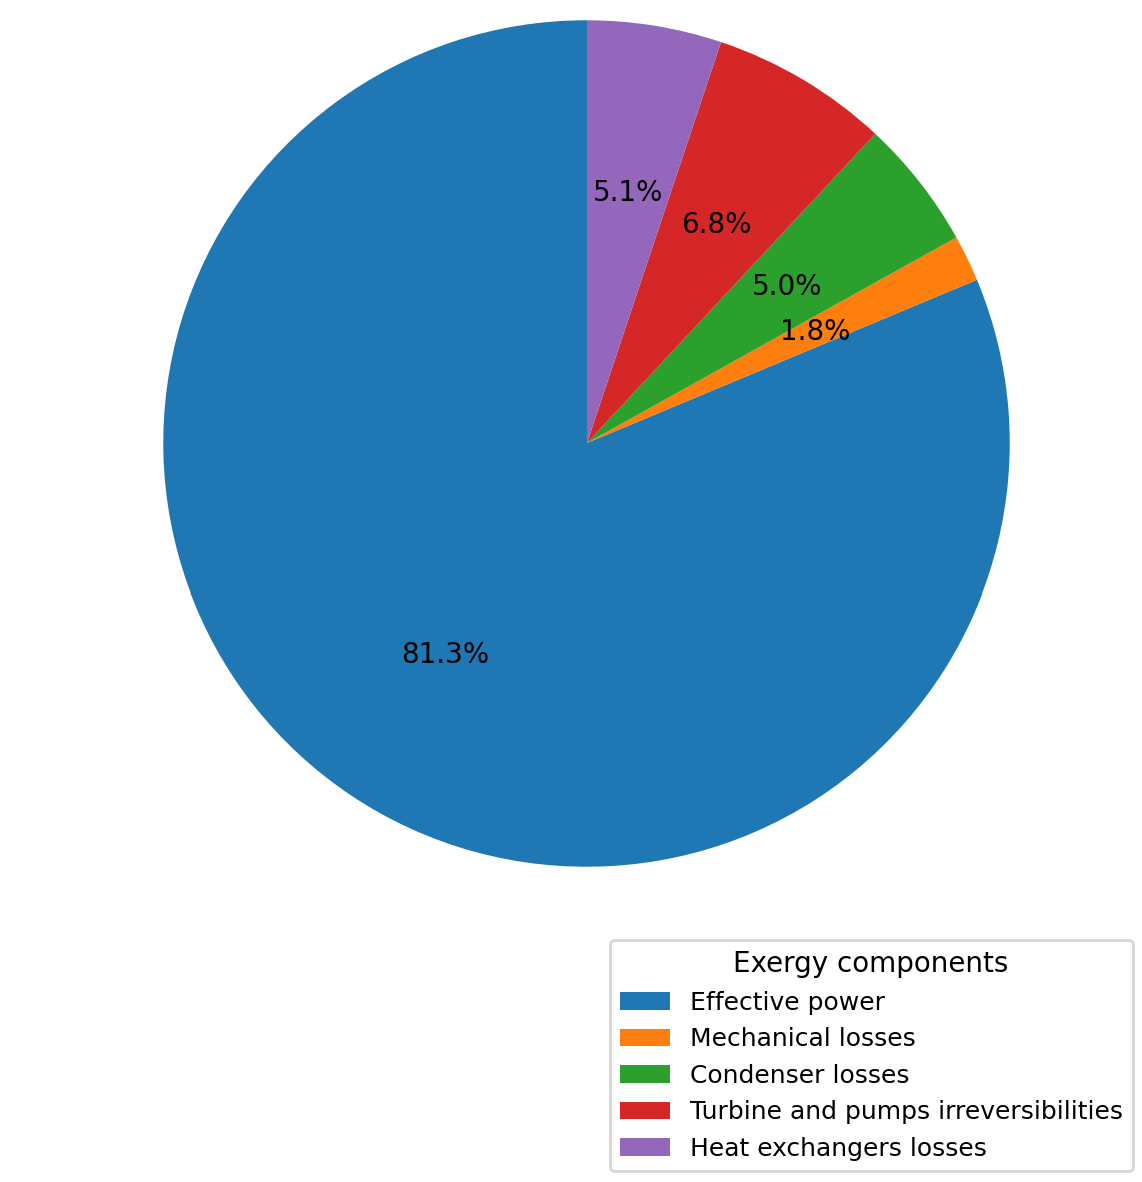
\includegraphics[width=0.7\textwidth]{Figures/pie_exergy.png}
        \caption{Exergy pie chart}
        \label{fig:exergy_pie_chart}
    \end{minipage}
\end{figure}